%% LaTeX Paper Template, Flip Tanedo (flip.tanedo@ucr.edu)
%% GitHub: https://github.com/fliptanedo/paper-template-2022

\documentclass[12pt]{article}

%!TEX root = paper.tex
%% FLIP’S PREAMBLE; 
%% Use FlipAdditionalHeader for project-specific packages & macros

% \pdfoutput=1 % for JHEP

%%%%%%%%%%%%%%%%%%%%%%%%%%
%%%  COMMON PACKAGES  %%%%
%%%%%%%%%%%%%%%%%%%%%%%%%%

\usepackage{amsmath}
\usepackage{amssymb}
\usepackage{amsfonts}
\usepackage{graphicx}
\usepackage[utf8]{inputenc}     % inspire bibs
\usepackage{aas_macros}				  % ads bibs
\usepackage{bm}                 % \boldsymbol
\usepackage{amsthm}
\usepackage{microtype}

%%%%%%%%%%%%%%%%%%%%%%%%%%%
%%%  UNUSUAL PACKAGES  %%%%
%%%%%%%%%%%%%%%%%%%%%%%%%%%

%% MATH AND PHYSICS SYMBOLS
%% ------------------------
\usepackage{slashed}				% \slashed{k}
\usepackage{mathrsfs}				% Weinberg-esque letters
\usepackage{bbm}					  % \mathbbm{1} conflict: XeLaTeX 
\usepackage{cancel}					
\usepackage[normalem]{ulem} % for \sout
\usepackage{youngtab}	    	% Young Tableaux

%% CONTENT FORMAT AND DESIGN
%% -------------------------
\usepackage[dvipsnames]{xcolor}
\usepackage[hang,flushmargin]{footmisc} % no footnote indent

\usepackage{fancyhdr}		% preprint number
\usepackage{lipsum}			% block of text 
\usepackage{framed}			% boxed remarks / Next time: use mdframed
                        % https://github.com/marcodaniel/mdframed/blob/master/mdframed.pdf
\usepackage{subcaption}	% subfigures
\usepackage{cite}			  % group cites
\usepackage{xspace}			% macro spacing


%% TABLES IN LaTeX
%% ---------------
\usepackage{booktabs}		% professional tables
\usepackage{nicefrac}		% fractions in tables,
\usepackage{multirow}		% multirow elements in a table
\usepackage{arydshln}		% dashed lines in arrays

%% ARRAY STRETCH: vertical spacing between rows
% \renewcommand{\arraystretch}{1.5} %% put this in main text

%% Other Packages and Notes
%% ------------------------
\usepackage[font=small]{caption} 	% caption font is small
\usepackage{float}         			  % for strict placement e.g. [H]


%%%%%%%%%%%%%%%%%%%%%%%%%%%%%%
%%%  DOCUMENT PROPERTIES  %%%%
%%%%%%%%%%%%%%%%%%%%%%%%%%%%%%

\usepackage[margin=2.5cm]{geometry} % margins
\graphicspath{{figures/}}			      % figure folder
\numberwithin{equation}{section}    % set equation numbering
% \usepackage{marginnote}             % for \marginnote{comment}
% \usepackage{mparhack}               % fix for \marginnote
% \usepackage{marginfix}              % fix for \marginnote
% \usepackage{adjustbox}              % to rescale elements



%% References in two columns, smaller
%% http://tex.stackexchange.com/questions/20758/
\usepackage{multicol}
\usepackage{etoolbox}
\usepackage{relsize}
\patchcmd{\thebibliography}
  {\list}
  {\begin{multicols}{2}\smaller\list}
  {}
  {}
\appto{\endthebibliography}{\end{multicols}}


% Change list spacing (instead of package paralist)
% from: http://en.wikibooks.org/wiki/LaTeX/List_Structures#Line_spacing
% alternative: enumitem package
\let\oldenumerate\enumerate
\renewcommand{\enumerate}{
  \oldenumerate
  \setlength{\itemsep}{4pt}
  \setlength{\parskip}{0pt}
  \setlength{\parsep}{0pt}
}

\let\olditemize\itemize
\renewcommand{\itemize}{
  \olditemize
  \setlength{\itemsep}{4pt}
  \setlength{\parskip}{0pt}
  \setlength{\parsep}{0pt}
}

%% FOR DRAFT EDITING AND DISCUSSION
\usepackage{lineno}
% \linenumbers          %% put this in main text


%%%%%%%%%%%%%%%%%%%%%%%%%%%
%%%  (RE)NEW COMMANDS  %%%%
%%%%%%%%%%%%%%%%%%%%%%%%%%%

%% FOR `NOT SHOUTING' CAPS (e.g. acronyms)
%% ---------------------------------------
\usepackage{scalefnt} 
\newcommand\acro[1]{{\footnotesize #1}}           % acronyms in footnote size


%% COMMON PHYSICS MACROS
%% ---------------------
\renewcommand{\tilde}{\widetilde}                 % tilde over characters
\renewcommand{\text}{\textnormal}	                % text in equations 
\renewcommand{\vec}[1]{\mathbf{#1}}               % vectors are boldface

%% Differential and differential/2pi
% \newcommand{\dbar}{d\mkern-6mu\mathchar'26}     % for d/2pi
\newcommand{\dbar}{d\mkern-6mu\mathchar'26\hspace{-.1em}}    
%% Best practice: Roman differential
\newcommand{\D}[1]{\ensuremath{\operatorname{d}\!{#1}}}
\newcommand{\Dbar}[1]{\operatorname{d}\mkern-10mu\mathchar'26\mkern-2mu{#1}}    % fixed spacing
\newcommand{\ket}[1]{\left|#1\right\rangle}       % <#1|
\newcommand{\bra}[1]{\left\langle#1\right|}       % |#1>
\newcommand*{\trans}{\mkern-1.5mu\mathsf{T}}      % transpose

%% COMMANDS FOR TEMPORARY COMMENTS
%% -------------------------------
\newcommand{\comment}[2]{\textcolor{red}{[\textbf{#1} #2]}}
\newcommand{\flip}[1]{{
	\color{green!50!black}
  \footnotesize
  [\textbf{\textsf{Flip}}: \textsf{#1}]
	}}


%% COMMANDS FOR TOP-MATTER
%% -----------------------
\newcommand{\email}[1]{\href{mailto:#1}{#1}}
\newenvironment{institutions}[1][2em]{\begin{list}{}{\setlength\leftmargin{#1}\setlength\rightmargin{#1}}\item[]}{\end{list}}


%% COMMANDS FOR LATEXDIFF
%% ----------------------
%% see http://bit.ly/1M74uwc
\providecommand{\DIFadd}[1]{{\protect\color{blue}#1}} %DIF PREAMBLE
\providecommand{\DIFdel}[1]{{\protect\color{red}\protect\scriptsize{#1}}}

%% REMARK: use latexdiff option --allow-spaces
%% for \frac, ref: http://bit.ly/1iFlujR
%% Errors with environments? https://tex.stackexchange.com/q/73224

%% USAGE: latexdiff draft.tex revision.tex > diff.tex

%%%%%%%%%%%%%%%%%%%%%
%%%  TITLE DATA  %%%%
%%%%%%%%%%%%%%%%%%%%%

%% PREPRINT NUMBER USING fancyhdr
%% Don't forget to set \thispagestyle{firststyle}
%% ----------------------------------------------
\renewcommand{\headrulewidth}{0pt} 	% no separator
\setlength{\headheight}{15pt} 		% min to avoid fancyhdr warning
\fancypagestyle{firststyle}{
	\rhead{\footnotesize%
	\texttt{\FlipTR}%
	}}

%% TOC overwrites fancyhdr, here's a fix
%% http://tex.stackexchange.com/questions/167828/
\usepackage{etoc}
\renewcommand{\etocaftertitlehook}{\pagestyle{plain}}
\renewcommand{\etocaftertochook}{\thispagestyle{firststyle}}			%% \usepackages
%!TEX root = paper.tex
%% Update the above with the appropriate root

%% Place additional project-specific macros, package calls here
%% These are called before FlipPreambleEnd.tex so that,
%% for example, they are called before hyperref


%% FIGURE SNIPPIT
% \begin{figure}[tb]
%     \centering
%     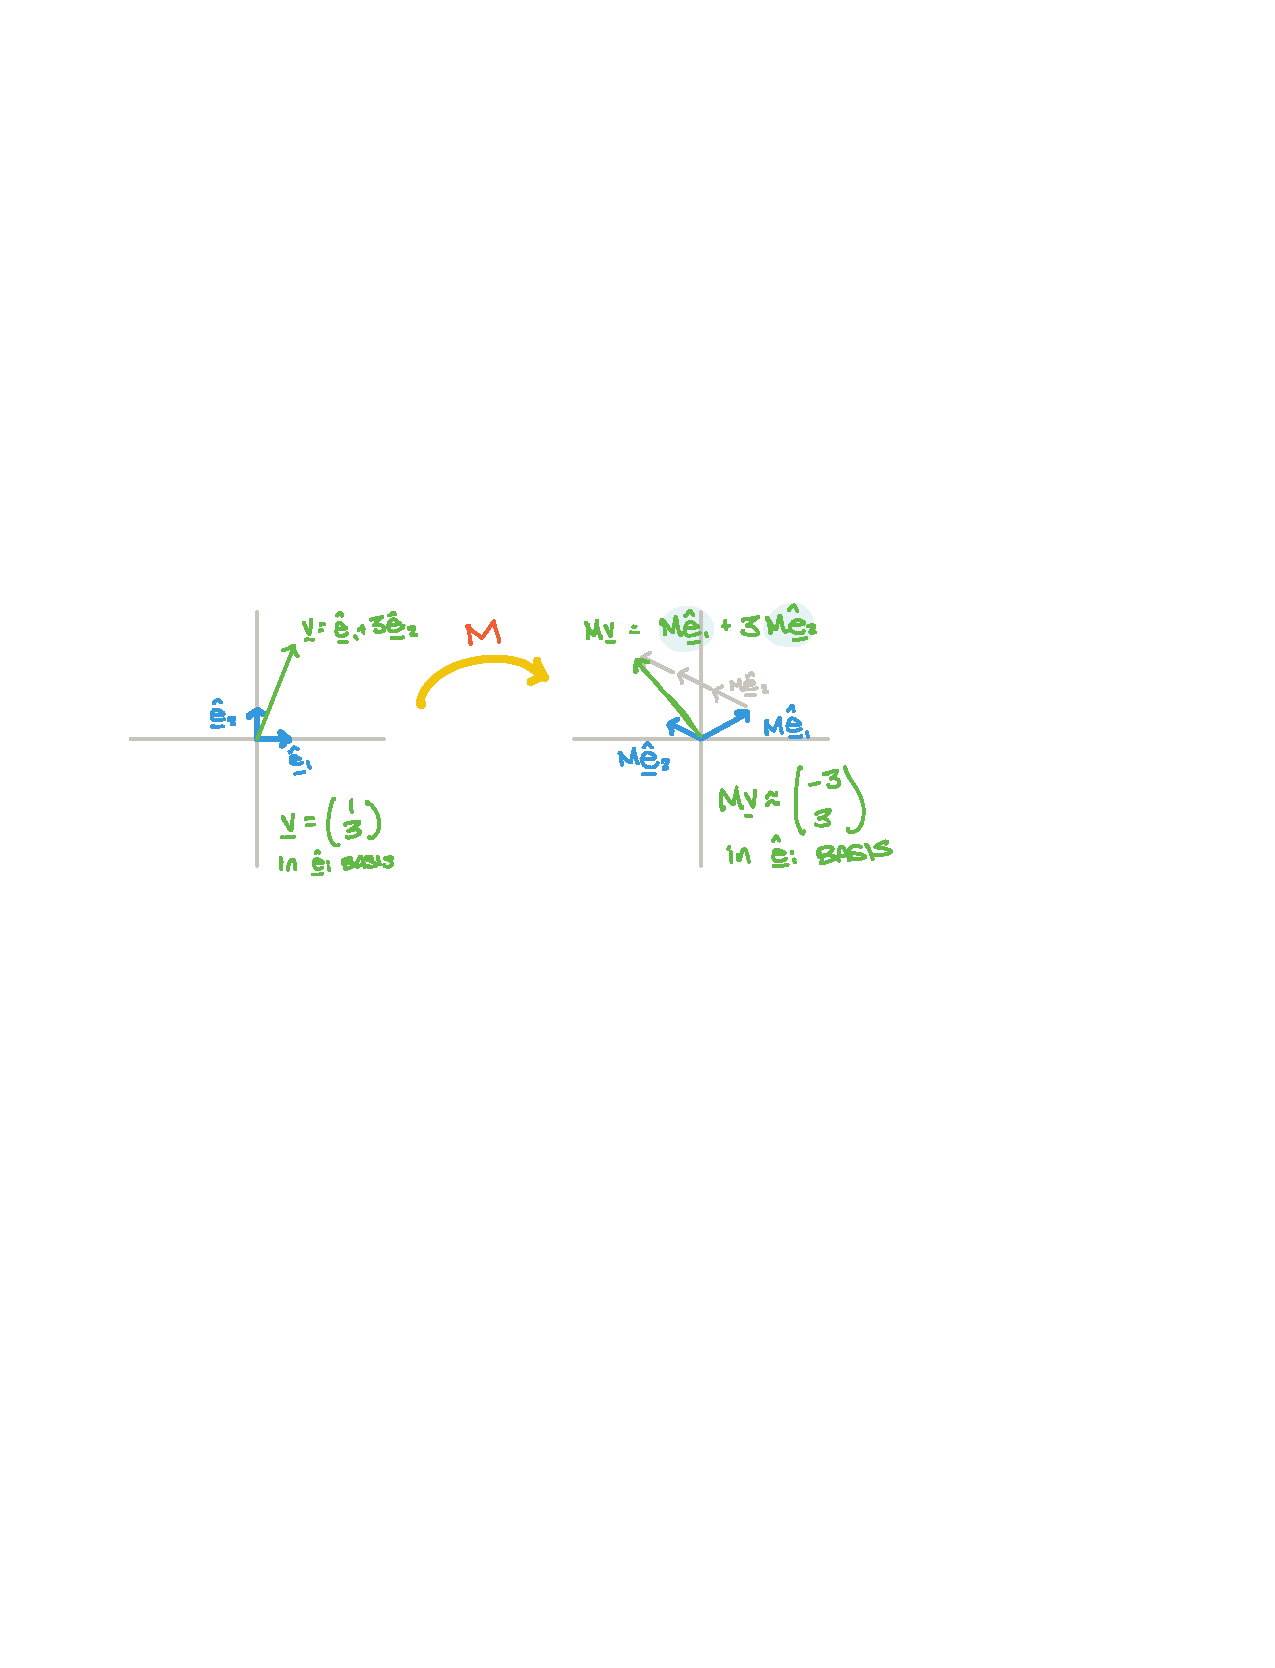
\includegraphics[width=.8\textwidth]{figures/maps_M.pdf}
%     \caption{.}
%     \label{fig:}
% \end{figure}

%% THEOREM ENVIRONMENTS


%% Because mdframed causes a bunch of warnings
%% https://tex.stackexchange.com/questions/64331/disable-warning-from-mdframed 
\usepackage{silence}
\WarningFilter{mdframed}{You got a bad break}
\WarningFilter{mdframed}{correct box splittet fails}



\newmdtheoremenv[
    skipabove=2em,
    skipbelow=2em,
    linewidth=5pt,
    linecolor=red!50!black,
    topline=false,
    rightline=false,
    bottomline=false
    ]{exercise}{Exercise}[section]


\newmdtheoremenv[
    skipabove=2em,
    skipbelow=2em,
    linewidth=5pt,
    linecolor=gray,
    topline=false,
    rightline=false,
    bottomline=false
    ]{example}{Example}[section]

\newmdtheoremenv[
    skipabove=2em,
    skipbelow=2em,
    linewidth=5pt,
    linecolor=blue,
    topline=false,
    rightline=false,
    bottomline=false
    ]{bigidea}{Key Idea}[section]
\newcommand{\bigidearef}{Key~Idea\xspace}
\newcommand{\bigidearefs}{Key~Ideas\xspace}

%% AMS Theorem version
% \newtheorem{exercise}{Exercise}[section]
% \newtheorem{example}{Example}[section]

%% Example: replace YourName with your name
\newcommand{\YourName}[1]{{	
	\color{blue!50!black}\footnotesize
	[\textbf{\textsf{YourName}}: \textsf{#1}]}}


\renewcommand{\tilde}{\widetilde}   % tilde over characters
\renewcommand{\vec}[1]{\mathbf{#1}} % vectors are boldface
\newcommand{\bas}[1]{\hat{\mathbf{#1}}} 	% basis vectors have hat
\newcommand{\row}[1]{\tilde{\mathbf{#1}}} 	% row vectors have tilde

% For matrices
\newcommand{\aij}[2]{^{#1}_{\phantom{#1}#2}}
\newcommand{\mat}[3]{#1\aij{#2}{#3}}
\newcommand{\pp}{\phantom{+}}
\newcommand{\inv}{^{-1}}


\usepackage{pifont}
	\newcommand{\cmark}{\ding{51}}%
	\newcommand{\xmark}{\ding{55}}%


%% COMMANDS FOR TEMPORARY COMMENTS
%% -------------------------------
\newcommand{\comment}[2]{\textcolor{red}{[\textbf{#1} #2]}}
\newcommand{\flip}[1]{{
	\color{green!50!black}
  \footnotesize
  [\textbf{\textsf{Flip}}: \textsf{#1}]
	}}

\newcommand{\correction}[2]{{
	\color{green!50!black}
  \footnotesize
  [\textbf{\textsf{Correction,~#1}}: \textsf{#2}]
	}}
 	%% Use this define additional macros
% %!TEX root = paper.tex
%% Update the above with the appropriate root


%% LISTINGS PACKAGE
%% https://www.overleaf.com/learn/latex/Code_listing
%% https://tex.stackexchange.com/a/350242
\usepackage{xcolor}
\usepackage[most]{tcolorbox}
\usepackage{listings}

\definecolor{white}{rgb}{1,1,1}
\definecolor{mygreen}{rgb}{0,0.4,0}
\definecolor{light_gray}{rgb}{0.97,0.97,0.97}
\definecolor{mykey}{rgb}{0.117,0.403,0.713}

\tcbuselibrary{listings}
\newlength\inwd
\setlength\inwd{1.3cm}

\newcounter{ipythcntr}
\renewcommand{\theipythcntr}{\texttt{[\arabic{ipythcntr}]}}

\newtcblisting{pyin}[1][]{%
  sharp corners,
  enlarge left by=\inwd,
  width=\linewidth-\inwd,
  enhanced,
  boxrule=0pt,
  colback=light_gray,
  listing only,
  top=0pt,
  bottom=0pt,
  overlay={
    \node[
      anchor=north east,
      text width=\inwd,
      font=\footnotesize\ttfamily\color{mykey},
      inner ysep=2mm,
      inner xsep=0pt,
      outer sep=0pt
      ] 
      at (frame.north west)
      {\refstepcounter{ipythcntr}\label{#1}In \theipythcntr:};
  }
  listing engine=listing,
  listing options={
    aboveskip=1pt,
    belowskip=1pt,
    basicstyle=\footnotesize\ttfamily,
    language=Python,
    keywordstyle=\color{mykey},
    showstringspaces=false,
    stringstyle=\color{mygreen}
  },
}
\newtcblisting{pyprint}{
  sharp corners,
  enlarge left by=\inwd,
  width=\linewidth-\inwd,
  enhanced,
  boxrule=0pt,
  colback=white,
  listing only,
  top=0pt,
  bottom=0pt,
  overlay={
    \node[
      anchor=north east,
      text width=\inwd,
      font=\footnotesize\ttfamily\color{mykey},
      inner ysep=2mm,
      inner xsep=0pt,
      outer sep=0pt
      ] 
      at (frame.north west)
      {};
  }
  listing engine=listing,
  listing options={
      aboveskip=1pt,
      belowskip=1pt,
      basicstyle=\footnotesize\ttfamily,
      language=Python,
      keywordstyle=\color{mykey},
      showstringspaces=false,
      stringstyle=\color{mygreen}
    },
}
\newtcblisting{pyout}[1][\theipythcntr]{
  sharp corners,
  enlarge left by=\inwd,
  width=\linewidth-\inwd,
  enhanced,
  boxrule=0pt,
  colback=white,
  listing only,
  top=0pt,
  bottom=0pt,
  overlay={
    \node[
      anchor=north east,
      text width=\inwd,
      font=\footnotesize\ttfamily\color{mykey},
      inner ysep=2mm,
      inner xsep=0pt,
      outer sep=0pt
      ] 
      at (frame.north west)
      {\setcounter{ipythcntr}{\value{ipythcntr}}Out#1:};
  }
  listing engine=listing,
  listing options={
      aboveskip=1pt,
      belowskip=1pt,
      basicstyle=\footnotesize\ttfamily,
      language=Python,
      keywordstyle=\color{mykey},
      showstringspaces=false,
      stringstyle=\color{mygreen}
    },
}


% amsthm details:


\newtheorem{exercise}{Exercise}[section]
\newtheorem{example}{Example}[section]

%!TEX root = paper.tex
%% These are packages that need to be called at the end of the preamble 
%% or else they may lead to potential package conflicts.

%%%%%%%%%%%%%%%%%%%
%%%  HYPERREF  %%%%
%%%%%%%%%%%%%%%%%%%

%% This package has to be at the end; can lead to conflicts
\usepackage[
	colorlinks=true,
	citecolor=green!50!black,
	linkcolor=NavyBlue!75!black,
	urlcolor=green!50!black,
	hypertexnames=false]{hyperref}

%%%%%%%%%%%%%%%%%%%%%%%%%%%%%%%%%%%%%%%%
%%%  Must be called after HYPERREF  %%%%
%%%%%%%%%%%%%%%%%%%%%%%%%%%%%%%%%%%%%%%%


\usepackage{orcidlink}			% orcid ID icon; after hyperref
\usepackage{cleveref}
\crefformat{equation}{(#2#1#3)}	% strip eq.~ 
\crefrangeformat{equation}{(#3#1#4\,--\,#5#2#6)} % strip eqs.~			%% packages that have to be at the end
\begin{document}

\newcommand{\FlipTR}{UCR-TR-2023-FLIP-00X} % (pdfsync may fail on 1st page)
	\thispagestyle{firststyle} 	% TR#; otherwise use \thispagestyle{empty}


%%%%%%%%%%%%%%%%%%%%%%%%
%%%  FRONTMATTER    %%%%
%%%%%%%%%%%%%%%%%%%%%%%%

\begin{center}
    {\huge \textbf{Linear Algebra for Physicists} \par}
    \vskip .5cm
    %!TEX root = paper.tex
%% Update the above with the appropriate root

%% This is the author list
%% We separate it to keep the main file clean; this is
%% not the part of the document that gets updated often.

\newcommand{\authorA}{Flip Tanedo}
\newcommand{\emailA}{flip.tanedo@ucr.edu}
\newcommand{\orcidA}{0000-0003-4642-2199}
\newcommand{\institutionA}{
		Department of Physics \& Astronomy, 
	    University of  California, Riverside, 
	    \acro{CA} 92521}

\newcommand{\authorB}{Your Name}
\newcommand{\emailB}{your.name@ucr.edu}
\newcommand{\orcidB}{0000-0003-4642-2200}
\newcommand{\institutionB}{
		Department of Physics \& Astronomy, 
	    University of  California, Elsewhere, 
	    \acro{CA} 99999}

\newcommand{\authorC}{Tu Nombre}
\newcommand{\emailC}{tu.nombre@ucr.edu}
\newcommand{\orcidC}{0000-0003-4642-2201}
\newcommand{\institutionC}{
		Department of Physics \& Astronomy, 
	    University of  California, Elsewhere, 
	    \acro{CA} 99999}

	\textbf{\authorA}%$^{a}$,
	% \textbf{\authorB}$^{b}$,
	% and
	% \textbf{\authorC}$^{c}$, 
	\\ 
	\texttt{\footnotesize \email{\emailA}}~\orcidlink{\orcidA}%,
	% \texttt{\footnotesize \email{\emailB}}~\orcidlink{\orcidB},
	% \texttt{\footnotesize \email{\emailC}}~\orcidlink{\orcidC}

	\vspace{-.8em}
    \begin{institutions}[1.7cm]
    \footnotesize
    { 
    	% $^{a}$
    	\textit{\institutionA} 
    	% \\ $^{b}$ \textit{\institutionB} 
    	% \\ $^{c}$ \textit{\institutionC} 
	}    
    \end{institutions}


\end{center}

\begin{abstract}
\noindent 
Lecture notes for Physics 17, a course on linear algebra in preparation for upper-division undergraduate physics coursework at \acro{UC R}iverside.
\end{abstract}

\small
\setcounter{tocdepth}{2}
\tableofcontents
\normalsize
%\clearpage


%%%%%%%%%%%%%%%%%%%%%
%%%  THE CONTENT  %%%
%%%%%%%%%%%%%%%%%%%%%

\section{Logistics}

At any time in this course, you should feel comfortable asking either of the following questions:
\begin{enumerate}
    \item Is it obvious that...?
    \item Why is this significant?
\end{enumerate}
The first question is the way to ask for on-the-spot clarification---I will either appreciate that I did not properly explain a subtle point, \emph{or} I will explain the intuition\footnote{Your sense of mathematical and physical intuition is incredibly valuable. This is one of the key traits that makes a physics training unique.} for why something should be obvious. The second question is a way to remind me that I may have \emph{lost sight of the forest for the trees}: I want this course to \emph{mathematically connect big ideas in physics}. Asking this question is a reminder that making those connections justifies the hard mathematical work we will put into the course.


Finally, I want to comment on the word \emph{obvious}. I write this often. It is somewhat dangerous because it can come off as being arrogant: \emph{this is so obvious to me, if you do not understand you must be deficient}. This is never the reason why I use that word. Instead, the word \emph{obvious} serves a very practical purpose. The goal of this class is not just to be able to ``do stuff'' (e.g.~diagonalize a symmetric matrix), but to also build that intuition that comes from a deeper understanding how the mathematics works. In this sense, every time I write the word \emph{obvious} it is a flag: I am saying something that---with the proper perspective---should be self-evident. If it is not self-evident, then you should stop to interrogate why it is not self-evident. Most likely there is something where a change in perspective may (1) make it obvious, and (2) in so doing deepen your understanding of the subject. So when you see the word `obvious,' I want you to do a quick check to confirm whether or not the statement is indeed obvious. If it is not, then welcome the opportunity to learn.\footnote{There is, of course, the possibility that what I have written is \emph{not} obvious. For example, if I have made a typo... in which case, please let me know.}

\section{Motivation}

Here are three incredibly significant equations in physics:
\begin{align}
    \vec{F} &= m\vec{a}
    &
    R_{\mu\nu} - \frac{1}{2}Rg_{\mu\nu} 
    &= \frac{8\pi G_\text{N}}{c^4} T_{\mu\nu}
    &
    \hat H |\Psi\rangle 
    &= E |\Psi\rangle \ .
    \label{eq:three:equations}
\end{align}
These are Newton's force law, Einstein's field equations, and the Schr\"odinger equation. They govern classical physics, general relativity, and quantum theory. 


Each equation looks rather unique: they seem to each be speaking their own mathematical language. Newton's law is written with boldfaced vectorial quantities $\vec{F} = (F_x, F_y, F_z)^T$ that should look very familiar to any physics undergraduate. Einstein's equation has these funny $\mu$ and $\nu$ indices on every term---have you seen these before? Do they look intimidating? If you ever want to make your equations look ``technical'' and ``physicsy,'' you should dress them up with indices. The Schr\"odinger equation has no indices, but instead has these funny angle-brackety things... and that $\hat H$ looks suspicious. Where did $H$ get a hat, and what is the content of this equation other than $\hat H = E$?

\emph{Each of these equations turns out to be a ``vectorial'' equation.} Each one is actually shorthand for a number of equations. Newton's equation is shorthand for three equations, one for each component. Einstein's equation is shorthand for 16 equations, one for each combination of the indices $\mu$ and $\nu$ that run over four values\footnote{The four values are the three directions of space and one direction of time.}. The Schr\"odinger equation is shorthand for an \emph{infinite} number of equations, one for each allowed energy of a quantum system.

The mathematical formalism that unifies these different ideas (and notations) of `vector' is called linear algebra. It may sound humble: after all, ``linear'' systems are \emph{easy}, aren't they? Did we not just spend years of our lives learning fancy things like \emph{calculus} and \emph{differential equations} to deal with functions that are more complicated than \emph{lines}? In some sense, yes: linear algebra is about lines and planes in different numbers of dimensions.\footnote{On the other hand: a good chunk of the calculus that we do is also implicitly linear. Physicists often Taylor expand and keep only the $\mathcal O(\varepsilon)$ term. Integration boils down to summing trapezoids whose angley-bits are given by the first derivative of a function... the linear component.} However, linear algebra turns out to be far more richer than what you may be used to from high school. 

In this course we will see how the three equations in \eqref{eq:three:equations} are connected by the mathematics of linear algebra. We will dive into the different notation and shamelessly pass between $\vec{v}$, $v^i$, and $\ket{v}$ to describe the same abstract vector. We will connect to the mathematical description of \emph{symmetry} and see how it is an underlying theme in our descriptions of nature. And we will do all of this in a way that will make the instructors of the linear-algebra-for-mathematicians course and linear-algebra-for-engineers course vomit a little in disgust. Consider that one of privileges of being a physicist.


\section{Basics}

\subsection{Pre-conceptions}

If this were a mathematics course, then we would start by very carefully defining words like \emph{vector} and \emph{matrix}. As a physics student, you already have a working definition of these words. It is probably something like this:
%
\begin{quote}
A vector has a magnitude and a direction. We write a vector as an array of three numbers arranged in a column. A matrix is an array of nine numbers arranged in a $3\times 3$ block. There is a rule for how to apply (multiply) the matrix to the vector to produce a new vector.
\end{quote}

The problem is that you already know too much to learn linear algebra as a mathematics student. You have already seen the tip of the iceberg and so have preconceptions about what vectors are and how they work. You may remember from freshman mechanics that forces are vectors. So are momenta and velocities. You may also recall the idea of a force field---like the electric field---which is actually a whole bunch of vectors: one for each point in space. Examples of matrices are a little more subtle: you may recall that you can represent rotations as matrices. Speaking of rotations, there was another thing that showed up called the moment of inertia \emph{tensor}. It looked like a matrix, but we never called it the ``moment of inertia matrix.'' What the heck is a tensor, anyway?

And so, you see that starting this course like a mathematics course could cause trouble. The mathematics professor would start by defining a vector. That definition will say nothing about magnitudes or directions, and will not even say anything about arrays of numbers. That definition will clash with the hard-earned intuition that you built from your physics education thus far. It will be perplexing, and may make you feel rather unhappy. What do these mathematicians know, anyway? Or maybe its the physics that is wrong, or have we just completely misunderstood everything and we are just now noticing that we are hopelessly lost? We begin to spiral into a black hole of confusion.

\begin{framed}
Fortunately, \emph{this is not a mathematics course.}
\end{framed}

As a consequence, we will not give a rigorous definition of a vector. We start with a familiar definition of vectors and lay out which qualities are general, and which properties are specific. Then we will come to appreciate the approximation that ``\emph{everything is a vector}.'' So let us start with something comfortably familiar, even though it constitutes only the simplest example of a vector.

\subsection{Real Three-Vectors}

Let us write $\vec{v}$ to be a vector. This is a standard convention for writing a vector. In this course we will use a few different notations for vectors according to convenience. Notation is neither physics nor mathematics, it is simply a shorthand for a physical or mathematical idea. 

% At this point, you may wonder \emph{what is a vector, anyway?} Maybe a vector is a column with three numbers that represent coordinates in three-dimensional space:
In fact, let us focus on a particular type of vector: \textbf{real three-vectors}. These are the familiar vectors that we can write as a column of three numbers that effectively represent the coordinates in three-dimensional space:
\begin{align}
    \vec{v} = 
    \begin{pmatrix}
        x\\ y\\ z
    \end{pmatrix} \ ,
\end{align}
where $x$, $y$, and $z$ are real numbers. These numbers are called the \textbf{components} of the vector $\vec{v}$.

\begin{exercise}
There is something very perverse about this ``vector.'' The variable names $x$, $y$, and $z$ imply that $\vec{v}$ is something that physicists like to call a ``position vector.'' If you say this to a mathematician they will vomit. By the end of this course, you should appreciate why the notion of a position vector makes no sense. \emph{Hint:} You may have some intuition for this already: a velocity vector tells you about the instantaneous motion of a particle relative to its present position. Try to write the analogous statement for a ``position vector.\footnote{I am not a mathematician, but you see that even I have to write ``position vector'' in condescending quotation marks. In lecture I use even more condescending air quotes.}''
\label{ex:position:vector}
\end{exercise}

This three-dimensional space is called [three-dimensional] \textbf{real space} and we write it as $\mathbbm{R}^3$. This is because a vector is an element of three-dimensional real space specified by \emph{three} real numbers. 

Three-dimensional real space is an example of a \textbf{vector space}, which is just a stupidly formal way of saying that it is where vectors live. Vectors are \emph{elements} of a vector space. A vector space is the set of all possible allowed vectors of a given type. For $\mathbbm{R}^3$, the vector space is composed of all possible triplets of real numbers. 


\begin{example} It should be no surprise that we can imagine real two-dimensional space, $\mathbbm{R}^2$. This is a vector space where each vector may be written as two real numbers. You can also imagine writing real four-dimensional space, $\mathbbm{R}^2$, or complex two dimensional space, $\mathbbm{C}^2$. 
\end{example}

From the above example, you should have some intuition for what the \textbf{dimension} of a vector space means: the dimension counts how many numbers you need to specify a vector. For real vector spaces, $\mathbbm{R}^d$, the dimension is the number $d$. We will always assume that $d$ is a positive integer.\footnote{The notion of a non-integer-dimensional space does show up occasionally. These do not even have to be particularly exotic: you can look up the dimension of a fractal.}

\subsection{Vectors and Numbers}

We now make some general statements about vector spaces. These apply to all vector spaces, not just $\mathbbm{R}^3$, but you can keep $\mathbbm{R}^3$ in mind as we go over them.

First we should make clear that there are now two different kinds of objects: \emph{vectors} and \emph{numbers}. We will have all sorts of notation for vectors, but let us write them with a boldfaced Roman letter for now, e.g.~$\vec{v}$. We typically write numbers as lowercase italicized Roman letters like $a$ or sometimes Greek letters like $\alpha$. 

You already know everything there is to know about numbers.\footnote{Formally, what I mean by `number' is what mathematicians call a \textbf{field}. This simply means some objects where one can add, subtract, multiply, and divide as you would expect. This term is a little tedious for us because physicists usually mean something else when they say `field.' Usually we mean something like the electric field or the field associated with the Higgs boson.} Most relevant is that you can multiply numbers with each other (including division, the inverse of multiplication) and you can add them together (including subtraction). For the first part of this course, we will focus on real numbers, $\mathbbm{R}$. Later we will also allow for complex numbers, $\mathbbm{C}$. 

Like numbers, vectors can be added and subtracted. In fact, vector arithmetic turns out to be very similar to `number arithmetic.' However, unlike numbers, there is no obvious definition for vector multiplication. This leads to the idea of \emph{defining} functions for various kinds of vector multiplication. Linear algebra is the study of a particular class of these functions. The dot product, for example, which takes two vectors and returns a number, is something we have to ``make up'' and attach to a vector space.

% What about vectors? Vectors have the following properties: 
% \begin{enumerate}
%     \item You can add vectors. This assumes that they are in the same vector space. The sum of two vectors is also a vector in the same vector space. 
%     \item Vector addition is associative. This means that in the sum $\vec{v}+\vec{w}+\vec{u}$, it does not matter if you add $(\vec{v}+\vec{w})$ first and then add $\vec{u}$, or if you take $\vec{v}$ and then add it to $(\vec{w}+\vec{u})$. This is the kind of `obvious' property that we tend to take for granted.
%     \item Vector addition is commutative. $\vec{v}+\vec{w} = \vec{w}+\vec{v}$. This is also kind of obvious. But recall that matrix multiplication is not commutative.
%     \item There is a zero vector, $\vec{0}$, that does leaves any other vector unchanged under addition. $\vec{v}+\vec{0} = \vec{v}$. This should be totally obvious. I bet you even know what the components of $\vec{0}$ are.
%     \item There is an additive inverse (negative vectors). If $\vec{v}$ is a vector, then $-\vec{v}$ is a vector and satisfies $\vec{v}+(-\vec{v}) = \vec{0}$.
%     \item You can multiply vectors by numbers. This is called rescaling or scalar multiplication. All the usual properties of multiplication by numbers holds: associativity, commutivity, distributive law.
% \end{enumerate}
% \begin{example}
% The first property implies that once you have identified one vector in a vector space, $\vec{v}$, then you can immediately have an infinite number of vectors. This is because $2\vec{v} = \vec{v}+\vec{v}$ must also be a vector. Then $3\vec{v} = 2\vec{v}+\vec{v}$ must also be a vector. And so forth.
% \end{example}
% Let us go over a few of these properties.

\subsection{Notation: Indices}

One theme in this course is that we will repeatedly refine our notation to suit our needs. Let us introduce an \emph{index} notation where we write the components of vectors $\vec{v}$ and $\vec{w}$ as follows:
\begin{align}
    \vec{v}
    &=
    \begin{pmatrix}
        v^1 \\ v^2 \\ v^3
    \end{pmatrix}
    &
    \vec{w}
    &=
    \begin{pmatrix}
        w^1 \\ w^2 \\ w^3
    \end{pmatrix} \ .
\end{align}
We see that a boldfaced Roman letter, $u$, corresponds to a vector. The \emph{components} of the vector are $u^1$, $u^2$, $u^3$. The ``$x$-component'' of $\vec{u}$ is called $u^1$: we use the same letter as the vector, but italicized rather than boldfaced. The upper index is \emph{not} some kind of power, it simply means ``the first component.'' 

\begin{example}
If you see $\vec{s}$, this is understood to be a vector that has multiple components. If it is a three-vector, it has three components. If you see $s^2$, then this means that this is the \emph{second component} of the vector $\vec{s}$. The component of a vector is a number. 
\end{example}

You may worry that this notation introduces ambiguity. If we see $q^2$, is this the square of some number $q$, or is it the second component of some vector $\vec{q}$? The answer depends on context. You should avoid choosing variable names where there is ever the potential for ambiguity. If you have a vector that you call $\vec{q}$, then do not use the letter $q$ for anything else.


% \subsection{Notation: Indices again}

% We can express this using index notation. 
You know from $\mathbbm{R}^3$ that you can add together any two vectors $\vec{v}$ and $\vec{w}$.
% 
Let us call this sum $\vec{u}$ so that $\vec{u}\equiv \vec{v}+\vec{w}$. Then we can succinctly write the components of $\vec{u}$ in one line:
\begin{align}
    u^i = v^i + w^i \ .
    \label{eq:u:v:plus:w:index}
\end{align}
The variable $i$ is called an \textbf{index}. What values does the index take? In this example, it is 
clear that \eqref{eq:u:v:plus:w:index} holds for $i=1,2,3$. That is, $i$ takes values from 1 to the dimension of the space. The typical convention is that we do not have to state the range of index values because it should be understood from the space itself. 

With that in mind, it should be clear that if $\vec{q}$ is the difference of two vectors, then the components of $\vec{q}$ may be succinctly written:
\begin{align}
\vec{q} &= \vec{v}-\vec{w}    
&
&\Leftrightarrow
&
q^i &= v^i - w^i \ .
\end{align}
In fact, as physicists we typically use the two statements above interchangeably. If you know the components of a vector, then you know the vector.



\subsection{Arithmetic and linear combinations}

All vector spaces allow addition and subtraction. This is defined component-wise. The sum of $\vec{v}$ and $\vec{w}$ is
\begin{align}
    \vec{v}+\vec{w} = 
    \begin{pmatrix}
        v^1 + w^1\\
        v^2 + w^2\\
        v^3 + w^3
    \end{pmatrix} \ .
\end{align}
What this means is that the \emph{sum} of two vectors is also a vector. That means that if $\vec{v}$ and $\vec{w}$ are vectors in $\mathbbm{R}^3$, then $(\vec{v}+\vec{w})$ is a vector in $\mathbbm{R}^3$. The components of the vector $(\vec{v}+\vec{w})$ are simply the sum of the components of $\vec{v}$ and $\vec{w}$. 
% 
A few formal properties that generalize to all vector spaces:
\begin{itemize}
    \item Vector addition is associative. This means that in the sum $\vec{v}+\vec{w}+\vec{u}$, it does not matter if you add $(\vec{v}+\vec{w})$ first and then add $\vec{u}$, or if you take $\vec{v}$ and then add it to $(\vec{w}+\vec{u})$. This is the kind of `obvious' property that we tend to take for granted.
    \item Vector addition is commutative. $\vec{v}+\vec{w} = \vec{w}+\vec{v}$. This is also kind of obvious. But recall that matrix multiplication is not commutative.
    \item There is a zero vector, $\vec{0}$, that does leaves any other vector unchanged under addition. $\vec{v}+\vec{0} = \vec{v}$. This should be totally obvious. The components of $\vec{0}$ are obviously all zero.
    \item There is an additive inverse (negative vectors). If $\vec{v}$ is a vector, then $-\vec{v}$ is a vector and satisfies $\vec{v}+(-\vec{v}) = \vec{0}$.
\end{itemize}
\begin{example}
The first property implies that once you have identified one vector in a vector space, $\vec{v}$, then you can immediately have an infinite number of vectors. This is because $2\vec{v} = \vec{v}+\vec{v}$ must also be a vector. Then $3\vec{v} = 2\vec{v}+\vec{v}$ must also be a vector. And so forth.
\end{example}

We get another type of operation ``for free'' with a vector space. This is called scalar multiplication or \emph{rescaling}.

% You can multiply vectors by numbers. This is called rescaling or scalar multiplication. All the usual properties of multiplication by numbers holds: associativity, commutivity, distributive law.









\subsection{Rescaling: multiplication by a number}

Another operation that exists in a vector space is rescaling: we multiply a vector by a number. 
Let $\alpha$ be a number. If you want to nitpick, let us restrict $\alpha$ to be a real number. If we have a vector $\vec{v}$ with components $v^i$, then $\alpha \vec{v}$ is also a vector.\footnote{``Also a vector'' means that it is also an element of the vector space; so $(\alpha\vec{v})$ is an element of $\mathbbm{R}^3$ is $\vec{v}$ is an element of $\mathbbm{R}^3$. } The components of $\alpha \vec{v}$ are
\begin{align}
    (\alpha v)^i = \alpha v^i \ ,
\end{align}
by which we mean
\begin{align}
    (\alpha\vec{v})
    =
    \begin{pmatrix}
        \alpha v^1 \\
        \alpha v^2 \\
        \alpha v^3 
    \end{pmatrix} \ .
\end{align}
The parenthesis on the left-hand side is sloppy notation to mean ``the vector that is the vector $\vec{v}$ rescaled by the number  $\alpha$.'' Another way of saying this is that there is a vector $\vec{w}\equiv \alpha\vec{v}$ whose components are $w^i = \alpha v^i$.

\begin{example}
Let us do one explicit example with numbers. Suppose the vectors $\vec{v}$ and $\vec{w}$ have components
\begin{align}
    \vec{v} &=
    \begin{pmatrix}
    \phantom{+}4.2\\
    -2.6\\
    \phantom{+}7.0        
    \end{pmatrix}
    &
    \vec{w} &=
    \begin{pmatrix}
    \phantom{+}5.3\\
    \phantom{+}2.1\\
    -2.5        
    \end{pmatrix} \ .
\end{align}
I can rescale each vector by different numbers: $\alpha = 10$, $\beta = 2$. We can consider the vector that comes from adding these rescaled vectors:
\begin{align}
    \vec{u} \equiv \alpha \vec{v} + \beta \vec{w} \ .
\end{align}
The second component of $\vec{u}$ is $u^2 = -26 + 4.2 = -21.8$.
\end{example}

At this point it is useful to define some jargon. A \textbf{scalar} is a number. This is in contrast to vectors (and matrices and tensors) which we can think of as arrays of numbers. In fact, every time you see the word scalar, you should just think ``number.'' Another name for `rescaling a vector by a number' is \emph{scalar multiplication}.



\subsection{Linear Combination and Span}

Based on our rules for vector space arithmetic, we know that if $\vec{v}$ and $\vec{w}$ are two vectors in our vector space and if $\alpha$ and $\beta$ are any two numbers, then
\begin{align}
    \alpha\vec{v} + \beta\vec{w} 
\end{align}
is also a vector in our vector space. We call any such sum---for any values of $\alpha$ and $\beta$---a \textbf{linear combination} of the vectors $\vec{v}$ and $\vec{w}$. You can of course generalize to the linear combination of more than two vectors, say
\begin{align}
    \alpha\vec{v} + \beta\vec{w} + \gamma\vec{u} \ .
\end{align}

Given some number of vectors---$\vec{v}$ and $\vec{w}$---you can ask what are all of the possible vectors that you can form from the linear combination of those vectors? This is a vector space.\footnote{You may want to convince yourself that this satisfies the requirements of vector space arithmetic.} We say that this vector space is \textbf{spanned} by the vectors $\vec{v}$ and $\vec{w}$. We call this vector space $\text{Span}(\vec{v},\vec{w})$. You can extend this to even more vectors, $\text{Span}(\vec{v}, \vec{w}, \vec{u},\cdots)$.

\begin{exercise}
Show that the vector space spanned by $\vec{v}$ and $\alpha\vec{v}$ is the same as the vector space spanned by $\vec{v}$.
\end{exercise}

\begin{exercise}
If $\mathbbm{R}^3$ is the space of vectors with three real components, argue that the span of any four vectors is at most $\mathbbm{R}^3$ but possibly a subset of $\mathbbm{R}^3$. Give an example where the span of four vectors is $\mathbbm{R}^2$. 
\end{exercise}

\subsection{Basis}

Let us push this idea further. For simplicity, let us focus on the two-dimensional plane, $\mathbbm{R}^2$. A vector in $\mathbbm{R}^2$ looks like this:
\begin{align}
    \vec{v} =
    \begin{pmatrix}
        v^1 \\ v^2
    \end{pmatrix} \ .
\end{align}
Any such vector may be written as the linear combination of the following two vectors:
\begin{align}
    \hat{\vec{e}}_1 &=
    \begin{pmatrix}
        1 \\ 0
    \end{pmatrix}
    &
    \hat{\vec{e}}_2 &=
    \begin{pmatrix}
        0 \\ 1
    \end{pmatrix} \ .
\end{align}
Indeed, it should be obvious that 
\begin{align}
    \vec{v} &= \alpha \hat{\vec{e}}_1 + \beta \hat{\vec{e}}_2
    & \text{with}&
    &\alpha &= v^1
    &\beta &= v^2 \ .
\end{align}
In other words, these `special' vectors $\hat{\vec{e}}_{1,2}$ satisfy:
\begin{enumerate}
    \item Any vector in $\mathbbm{R}^2$ may be written as a linear combinations of $\hat{\vec{e}}_{1,2}$. We showed this because $\vec{v}$ in the above discussion could be any vector in $\mathbbm{R}^2$. Thus $\text{Span}(\hat{\vec{e}}_{1},\hat{\vec{e}}_{1})=\mathbbm{R}^2$.
    \item The coefficients in the linear combination are precisely the components of the vector $\vec{v}$. Soon we will see that this observation is actually backwards: it is the choice that $\hat{\vec{e}}_{1}$ are special that defines the components of a vector.
\end{enumerate}

It should be obvious that any pair of vectors that ``aren't pointing in the same direction'' can span the entire space $\mathbbm{R}^2$. 
\begin{exercise}
What does ``aren't pointing in the same direction'' mean in this context? Use $\vec{v}$ and $\alpha\vec{v}$ in your answer.
\end{exercise}
We could try a different pair of vectors and consider its linear combinations:
\begin{align}
    \vec{f}_1 &=
    \begin{pmatrix}
        1\\1
    \end{pmatrix}
    &
    \vec{f}_2 &=
    \begin{pmatrix}
        0\\1
    \end{pmatrix} \ .
\end{align}
Then the vector $\vec{v}$ may be written as $\vec{v} = \alpha \vec{f}_1+ \beta\vec{f}_2$. To find $\alpha$ and $\beta$, we can simply plug in the components of $\vec{v}$ and $\vec{f}_{1,2}$ so that:
\begin{align}
    v^1 &= \alpha -\beta
    &
    v^2 &= \alpha \ .
\end{align}
In other words,
\begin{align}
    \vec{v} = (v^2) \vec{f}_1 + (v^2 - v^1)\vec{f}_2 \ .
\end{align}
These coefficients $\alpha = v^2$ and $\beta = v^2 - v^1$ may be written  in shorthand. Let's suggestively write
\begin{align}
    \vec{v} = 
    \begin{pmatrix}
        v^2\\
        v^2 - v^1
    \end{pmatrix}_f \ ,
\end{align}
where we use the subscript $f$ to mean ``coefficients with respect to $\vec{f}_{1,2}$. This looks just like a two-component vector, doesn't it?

\begin{exercise}
Let $\vec{v} \in \mathbbm{R}^2$ be the following vector in two-dimensional real space:
\begin{align}
    \vec{v}=
    \begin{pmatrix}
        3\\2
    \end{pmatrix} \ .
\end{align}
Here are two vectors that span $\mathbbm{R}^2$:
\begin{align}
    \vec{f}_1 &=
    \begin{pmatrix}
        2\\1
    \end{pmatrix}
    &
    \vec{f}_2 &=
    \begin{pmatrix}
        -1\\0
    \end{pmatrix} \ .
\end{align}
What are the coefficients $\alpha$ and $\beta$ so that $\vec{v} = \alpha \vec{g}_1 + \beta \vec{g}_2$?  \textsc{Answer}: $\alpha = 2$ and $\beta = 1$. 
\end{exercise}


What we're getting at is the following.  Define a set of vectors that span a space. We will call this set of vectors a \textbf{basis} of that space. Any vector in the space can be written as a linear combination of basis vectors. For example, if $\vec{b}_{1,2}$ are a basis of $\mathbbm{R}^2$, then for any vector $\vec{v}\in\mathbbm{R}^2$ we may write
\begin{align}
    \vec{v} = \alpha \vec{b}_{1} + \beta \vec{b}_2 \ .
\end{align}
Then we have encoded all of the data of vector $\vec{v}$ into the coefficients $(\alpha, \beta)$. 

\flip{I am here}


%  we can define any vector of that space by listing the coefficients of the basis vectors in the linear combination that 

% For example, the vectors $\hat{\vec{e}}_{1}$ are a basis of $\mathbbm{R}^2$. In fact, the vectors $\vec{f}_{1,2}$ are also a basis for $\mathbbm{R}^2$. So are the pair $\vec{g}_{1,2}$. 





\subsection{Operations that are not (yet) allowed}

In these definitions, we make a big deal about how the sum of two vectors \emph{is also a vector}. Or how the rescaling of a vector by a number \emph{is also a vector}. This is in contrast to operations that are either not allowed or that do not produce vectors. An example of an operation that is not allowed is adding together vectors from two different vector spaces. The following proposed sum of a vector in $\mathbbm{R}^3$ with  a vector in $\mathbbm{R}^2$ does not make sense:
\begin{align}
    \begin{pmatrix}
        v^1\\ v^2 \\v^3
    \end{pmatrix}
    +
    \begin{pmatrix}
        w^1\\ w^2 
    \end{pmatrix}
    =
    \; ?
\end{align}
If you find yourself adding vectors from two different vector spaces, then you have made a mistake.

Another operation that requires care is rescaling a real vector by a complex number. If $\vec{v}$ is a vector in $\mathbbm{R}^3$ and we try to multiply it by a complex number, $\alpha = 2+3i$, then the resulting ``vector'' is not a vector in $\mathbbm{R}^3$:
\begin{align}
    (\alpha\vec{v})^i = (2+3i)v^i \notin \mathbbm{R} \ ,
\end{align}
that is: the components of $\alpha\vec{v}$ are not real numbers, and so this cannot be an element of aa vector space that is \emph{defined} to have real components. Later on we will generalize to the case of \emph{complex vector spaces}, but we will treat that with some care.\footnote{If you want to be fancy, you can replace `number' with the mathematical notion of a field. Both the real numbers and the complex numbers are examples of fields. In my mind a field is just a class of number, though mathematicians have fancier definitions.}

Thus far, we have introduced the \emph{nouns} of this course: vectors. We have identified a few \emph{verbs} that let us do things with these vectors:
\begin{enumerate}
    \item Addition takes two vectors in a vector space and returns a vector in the same vector space. 
    \item Rescaling takes a vector and a number and returns a vector in the same vector space.
\end{enumerate}
We can rewrite this in the language of \emph{mappings} (or \emph{functions}) as follows. Let $V$ be a vector space, say $V=\mathbbm{R}^3$. Let us write $\mathbbm{R}$ mean [real] numbers. Then the above statements tell us that addition and rescaling can be thought of as maps:
\begin{enumerate}
    \item Vector addition: $V\times V \to V$
    \item Rescaling: $V\times \mathbbm{R} \to V$ \ .
\end{enumerate}
Do not be intimidated by the $\times$ symbol here. This ``mapping'' notation means nothing more and nothing less than the statements above.

We now know everything there is to know about the vector space $\mathbbm{R}^3$. We want to learn more about functions (maps) that involve this vector space. How can we combine vectors and numbers to produce other vectors and numbers? What about more complicated objects like matrices and tensors? 


\subsection{Euclidean three-space}

You may object: \emph{wait! I know there are more things you can do with three-vectors!} You remember that there are two types of vector multiplication that we use in physics. The \textbf{dot product} and the \textbf{cross product}. 

In $\mathbbm{R}^3$, the \textbf{dot product} is a map $V\times V \to \mathbbm{R}$. That means it takes two vectors and returns a number. The particular number that it returns is typically \emph{defined} to be
\begin{align}
    \vec{v} \cdot \vec{w} 
    = \sum_i v^i w^i  
    = v^1w^1 + v^2 w^2 + v^3w^3 \ .
    \label{eq:euclidean:3d:metric:intro}
\end{align}
The dot product generalizes in linear algebra. It is often called an \textbf{inner product} or a \textbf{metric} and has a few different notations that we will meet. What is important is that this dot/inner product is an \emph{additional} mathematical function that we attach to a vector space. 

Three-dimensional real space combined with the dot product/inner product/metric \eqref{eq:euclidean:3d:metric:intro} is called Euclidean three-space. In general, a vector space combined with a `dot product' is called a \textbf{metric space}. The word metric should invoke some etymological notion of measurement of distance. Indeed, the dot product is a tool that tells us how `close' two vectors are to one another---though it is not yet obvious how.

\begin{example}
Let $\mathbf{r}=(x,y,z)$ be a ``position vector'' of a point relative to the origin.\footnote{It is dangerous to use the phrase ``position vector,'' see Exercise~\ref{ex:position:vector}.} Then the distance of the point from the origin is
\begin{align}
    d = \sqrt{\vec{r}\cdot\vec{r}} =
    \sqrt{x^2+y^2 +z^2} \ .
    \label{eq:distance:in:space}
\end{align}
This gives a notion of how the dot product is related to measuring distances, but it turns out to be a bit of a red herring! The real sense in which the dot product measures the `closeness' of two vectors is the sense in which it defines an angle between those vectors. (See below.)
\end{example}

The \textbf{cross product} is a different story. You may remember the cross product from such hits as\footnote{\url{https://tvtropes.org/pmwiki/pmwiki.php/Main/YouMightRememberMeFrom}} angular momentum, $\vec{r}\times\vec{p}$. It looks like a map that takes two vectors and spits out another vector, $V\times V \to V$. Indeed, this is the case in Euclidean three-space. However, it had some funny properties compared to the dot product. For example, there was something weird with the order of the two vectors: $\vec{a}\times \vec{b}  = - \vec{b}\times \vec{a}$. It is also a bit funny that the direction of the output vector is completely different\footnote{The technical meaning of `completely different' is \emph{orthogonal}, which we define below with the help of the metric.} from the directions of the input vectors. It will turn out that this product does not generalize as simply as the dot product, though there is a generalization called the \textbf{wedge product} which is outside the scope of this course.\footnote{That is not to say that the wedge product is not relevant in phsyics. The wedge product features prominently in a mathematical field called \textbf{differential geometry}, which is in turn the framework for general relativity. The wedge product is related to defining volumes and integration measures.}

\begin{exercise}
Define the generalization of the Euclidean three-space metric to Euclidean space in $d$ dimensions. (Easy.)
\end{exercise}

\begin{exercise}
Try to define a generalization of the cross product in two-dimensional Euclidean space. Reflect on why this is much less natural than the generalization of the dot product. 
\end{exercise}

\subsection{Length in Euclidean three-space}

Euclidean three-space is real space combined with the Euclidean dot product, \eqref{eq:euclidean:3d:metric:intro}. The [Euclidean] \textbf{magnitude} (length) of a three vector $\vec{v}$ as $|\vec{v}|$ in Euclidean three-space. The magnitude is defined to be
\begin{align}
    |\vec{v}| = \sqrt{\vec{v}\cdot\vec{v}} \ .
\end{align}
This definition generalizes to Euclidean $d$-dimensional space with the appropriate generalization of the dot product.

\begin{example}
Consider the vector
\begin{align}
    \vec{v} = 
    \begin{pmatrix}
    \phantom{+}3\\-4\\\phantom{+}0    
    \end{pmatrix}
\end{align}
in Euclidean three-space. The magnitude of $\vec{v}$ is $|\vec{v}| = 5$.
\end{example}


Some references prefer to use the double bar notation, $||\vec{v}||$ for the length of a vector. This is to distinguish it from the absolute value of a number, $|-3| = 3$. We will be even more perverse: sometimes we will write $v$ to mean the magnitude of $\vec{v}$ when there is no ambiguity.

\begin{example}
Consider the vector
\begin{align}
    \vec{v} = 
    \begin{pmatrix}
    -1\\ \phantom{+}3\\ \phantom{+}2
    \end{pmatrix} \ .
\end{align}
Then the \emph{magnitude} of $\vec{v}$ is $|\vec{v}|=\sqrt{14}$. We could also write this as $v = \sqrt{14}$, but we should be careful when we write things like $v^2$ which could either mean the second component of $\vec{v}$---which is $3$---or the square of the magnitude---which is 14. 
\end{example}


We see that the dot product (metric) allows us to define length. Because the length of a vector is a number, we can divide the vector $\vec{v}$ by its its length $|\vec{v}|$ to obtain a \textbf{unit vector}, $\hat{\vec{v}}$:
\begin{align}
    \hat{\vec{v}} = \frac{1}{|\vec{v}|}\vec{v} \ .
    \label{eq:eg:v:340}
\end{align}
The right-hand side is simply scalar multiplication by $|\vec{v}|^{-1}$. Unit vectors are useful for identifying directions.

\begin{example}
In grade school one may have learned that a vector is an arrow that has a magnitude and a direction. Unit vectors encode the `direction' of a vector.
\end{example}

\begin{example}
Let $\vec{v}$ be defined as in \eqref{eq:eg:v:340}. The unit vector associated with $\vec{v}$ is
\begin{align}
    \hat{v} = 
    \begin{pmatrix}
        \phantom{+}3/5 \\
        -4/5\\
        0
    \end{pmatrix} \ .
\end{align}

\end{example}


\subsection{Angles in Euclidean three-space}

Let $\vec{v}$ and $\vec{w}$ be two vectors in Euclidean three-space. The [Euclidean] angle between these two vectors, $\theta$, is 
\begin{align}
    \cos\theta \equiv \hat{\vec{v}}\cdot\hat{\vec{w}} = \frac{\vec{v}\cdot\vec{w}}{|\vec{v}||\vec{w}|} \ .
\end{align}
\begin{exercise}
Confirm that this matches the definition of the angle between two vectors that you learned in your youth.
\end{exercise}
The above definition of the angle between two vectors is general for any metric space---that is, a vector space equipped with a dot product. 

\begin{example}
The angle between two vectors defines the sense in which two vectors are close to one another. This is the sense in which the dot product (metric) lets you measure the ``distance'' between two vectors. Note that this is completely different from the notion of distance between two points in space, \eqref{eq:distance:in:space}. 
\end{example}

\section{Index Notation and Summation Convention}

There's something that physicists do that tend to drive mathematicians crazy: we write a generic \emph{component of a vector} and refer to it as if it were the vector itself. It is a fairly harmless peccadillo:\footnote{There are times when you can get into trouble if you drink your own Kool Aid, so to speak. The reason is that the \emph{component} $v^i$ is simply a number, whereas $\vec{v}$ is a vector. Some manipulations are only allowed for numbers and not vectors, and you should be clear that you mean `the component $v^i$' if you are treating it like a number, and not `the \emph{vector} whose components are $v^i$.' See Example~\ref{eg:moving:coefficients:around}.} if I say ``the vector $v^i$,'' then it is not hard to guess that I mean ``the vector $\vec{v}$ which has components that I label $v^i$.''

The reason why we have this culture is that this index notation ends up being so damn convenient. In addition to vectors, we will have other objects that have indices: dual vectors, matrices, and tensors. When we write everything in with indices, we can ``see'' properties of these objects that are not obvious without the indices. Specifically, we can see \emph{how an object transforms under symmetries}. In this course, we will focus on \emph{rotations} of vectors and their generalizations.  


There's a second reason why indices are convenient: they allow us to use \textbf{Einstein summation convention}. This is a notational shortcut that introduces upper and lower indices to convey sums. Consider, for example, the ``matrix multiplication'' of a row vector $\row{w}$ on a column vector $\vec{v}$. Nevermind the formal definition of ``row vector'' as opposed to ``column vector.'' Let's just write it out in components where it is obvious for $\mathbbm{R}^3$
\begin{align}
    \row{w}
    &=
    \begin{pmatrix}
        w_1 & w_2 & w_3
    \end{pmatrix}
    &
    \vec{v}
    &=
    \begin{pmatrix}
        v^1 \\ v^2 \\ v^3
    \end{pmatrix}
    &
    \row{w}\vec{v}
    &= w_1v^1 + w_2v^2+w_3v^3 \ .
\end{align}
The final expression is familiar, right? It follows the usual rules of matrix multiplication for a matrix that happens to be one row and three columns. We notice that we chose to write the components of $\row{w}$ with lower indices---this is the convention. Row vectors (which have many names) have indices written as subscripts while column vectors have indices written as superscripts. There is no mathematics here, just a choice of notation. The result of the multiplication is simply a number, which we can write as a sum:
\begin{align}
    \row{w}\vec{v}
    &= \sum_{i=1}^3 w_iv^i
    \equiv w_iv^i \ .
    \label{eq:row:w:on:vec:v}
\end{align}
On the right-hand side we have \emph{defined} the summation convention: \emph{whenever there is exactly one upper index and exactly one lower index with the same letter, we should understand that there is a sum over that index over all of its allowed values.} We call pairs of repeated indices where one is upper and one is lower \textbf{contracted indices}.


The value $w_iv^i$ is simply a number. It is not a vector. It does not have any ``vectorial'' (tensorial) structure. It is not an element of the vector space $\mathbbm{R}^3$. It does not transform under rotations. It is \emph{just a number}. In other words, $w_iv^i$ behaves like an object with \emph{no indices}. Contracted indices ``cancel each other out.''

This is significant because we will see that indices tell us how objects transform. Evidently, column vectors and row vectors transform differently since one has an upper index and one has a lower index. Further, when we contract the two indices, we end up with something with no indices: a number that does not transform at all. This may seem like notational overkill---trust me, it is worth building this notation now. We will use it over and over.

\begin{example}
Matrices $M$ have the following index structure: $M\aij{i}{j}$. There is a first index and a second index---the order matters. The first index is upper, and the second index is lower. Matrix multiplication boils down to a contraction of indices:
\begin{align}
    (M\vec{v})^i = M\aij{i}{j}v^j \ .
    \label{eq:matrix:mult:ith:comp}
\end{align}
Let us read this equation carefully. First, $M\vec{v}$ is a vector. The $i^\text{th}$ component of this vector is $(M\vec{v})^i$. How is this related to the components of $M$ and $\vec{v}$? The right-hand side tells us that we simply take the sum:
\begin{align}
    M\aij{i}{j}v^j = 
    M\aij{i}{1}v^1 + M\aij{i}{2}v^2  + M\aij{i}{3}v^3 \ .
\end{align}
\end{example}
\begin{example}
From the above example, you can then excuse the glib statement: ``the \emph{vector} $M\aij{i}{j}v^j$.'' As we explained above, $M\aij{i}{j}v^j$ is not a vector, but a component of a vector. However, the point is that even though there are three indices, two of them are contracted so the object effectively only has one upper index. This is the index structure of a vector.
\end{example}

\begin{exercise}
Consider the following vector, row vector, and matrix:
\begin{align}
    \vec{v} &=
    \begin{pmatrix}
     1 \\ 2 \\ 3   
    \end{pmatrix}
    &
    \row{w} &=
    \begin{pmatrix}
        4&5&6
    \end{pmatrix}
    &
    M&=
    \begin{pmatrix}
        1 & 2 & 3 \\
        4 & 5 & 6 \\
        7 & 8 & 9
    \end{pmatrix} \ .
\end{align}
These have index structure $v^i$, $w_i$, and $M\aij{i}{j}$ respectively. Note that the first index of a matrix is the row and the second is the column, thus $M\aij{1}{2} = 2$ while $M\aij{2}{1} = 4$. Calculate the following: $(wM)_2$, $(Mv)^1$, $(MM)\aij{1}{2}$. Here $MM$ is understood to be the square of the matrix $M$, $(M^2)\aij{i}{j} = M\aij{i}{k}M\aij{k}{j}$.
\end{exercise}

\begin{example}\label{eg:moving:coefficients:around}
It should be clear that
\begin{align}
    w_i M\aij{i}{j} = 
    w_1 M\aij{1}{j} + w_2 M\aij{2}{j} + w_3 M\aij{3}{j}
    = 
    M\aij{1}{j}w_1  + M\aij{2}{j}w_2 + M\aij{2}{j}w_2
    =
    M\aij{i}{j}w_i \ .
\end{align}
After all, each of the components $w_i$ and $M\aij{i}{j}$ are simply numbers. However: even though $w_i M\aij{i}{j} = M\aij{i}{j}w_i$, it is \emph{completely incorrect} to say $\row{w}M = M\row{w}$. This is because $\row{w}$ and $M$ are \emph{tensorial} (vector-y) objects. The order of their `multiplication' matters. You can see this from the matrix notation.
\begin{align}
    \row{w}M &= 
    \begin{pmatrix}
        4&5&6
    \end{pmatrix}
    \begin{pmatrix}
        1 & 2 & 3 \\
        4 & 5 & 6 \\
        7 & 8 & 9
    \end{pmatrix}
    &
    M\row{w} &=
    \begin{pmatrix}
        1 & 2 & 3 \\
        4 & 5 & 6 \\
        7 & 8 & 9
    \end{pmatrix}
    \begin{pmatrix}
        4&5&6
    \end{pmatrix} \ .
\end{align}
The first multiplication gives a row vector, as you expect since $(wM)_j$ has one lower index. The second multiplication does not even make sense. What we see is that expressions like $w_i M\aij{i}{j} = M\aij{i}{j}w_i$ are valid as long as you are only talking about the components. The glib ``physicist slang'' of replacing a component by its vector/matrix/tensor can get you into trouble if you have moved components around in a way that is only allowed for numbers, but not vectory-things.
\end{example}

Since the language is now becoming cumbersome, let us define the word \textbf{tensorial} to mean an object with indices. This will replace the phrase ``vectory'' in our notes.

\section{Ket Notation}

Quantum mechanics has a completely different notation for vectors. Rather than $\vec{v}$, we write $\ket{v}$. This is called a \emph{ket}. The reason for this is that we write row vectors as $\row{w} = \bra{w}$. We call this object a \emph{bra}. Then the ``matrix multiplication'' $\row{w}\vec{v}$ from \eqref{eq:row:w:on:vec:v} is succinctly written $\langle w|v\rangle$. The pun is that this is a `bra--ket' or a \emph{bracket}. At the moment we do not have much use for bra and ket notation, but it is useful to establish this notation early on. It will soon be \emph{very} convenient. To summarize:
\begin{align}
    \text{column vector:}\quad \vec{v} &= \ket{v}
    &
    \text{row vector:}\quad \row{w} &= \bra{w}
\end{align}
There is no special notation for matrices, $M$. If you really want to be fancy, though, you can give matrices a hat and write them $\hat M$. This is really only important if you need to distinguish between a matrix and a number that happens to have a similar variable name. 

\begin{example}
As an example where the `hat' notation comes in handy, recall the Schr\"odinger equation in \eqref{eq:three:equations}:
\begin{align}
    \hat H \ket{\Psi} = E \ket{\Psi} \ .
\end{align}
The $\hat H$ has a hat because it is a matrix. The $E$ does not have a hat because it is a number. Does this information give the equation more significance? Obviously $\hat H \neq E$ since these are two completely different classes of objects. The equation is an equality between two vectors, $\ket{\Psi}$. Evidently, when the matrix $\hat H$ hits $\ket{\Psi}$, you end up with a new vector that is simply a rescaling of $\ket{\Psi}$. We say that $\ket{\Psi}$ is an \emph{eigenvector} of $\hat H$. 
\end{example}



\section{Matrices and Linear Transformations}

Vectors are the `nouns' in linear algebra. The word `linear' refers to the the \emph{verbs}. That is: we would like to act on vectors. 


\subsection{Jargon}
Let us introduce some jargon here. Rather than formal definitions, we give practical ``physicist's'' definitions.\footnote{If we do something less formally, we say that we are physicists, not mathematicians. If we choose to be more highbrow, then we say that we are physicists, not engineers.} You can look up proper definitions in your favorite mathematics textbook.  The following words are closely related: function, map, transformation. I often use them interchangeably, though this is rather sloppy.  

A \textbf{function} is a mathematical machine that takes some inputs and produces some output. The inputs can be numbers, vectors, or more sophisticated objects. The outputs may also be numbers, vectors, or more sophisticated objects. The outputs do not have to be the same type of object as the inputs---in general they are not.
% 
A function that takes one input and returns one output is called a \textbf{map}. 
% 
A map that takes one type of object and returns the same type of object is called a \textbf{transformation}. Mathy-folks like to draw diagrams like Fig.~\ref{fig:Linear Transformation}.

\begin{example}
The dot product is a \textbf{function} that takes in two vectors and outputs a number.
\end{example}
\begin{example}
The magnitude is a \textbf{map} that takes a vector and returns a number.
\end{example}
\begin{example}
The map that takes a vector and returns its unit vector is a \textbf{transformation}: it is a function that takes a vector and returns a vector.
\end{example}

\begin{figure}[tb]
    \centering
    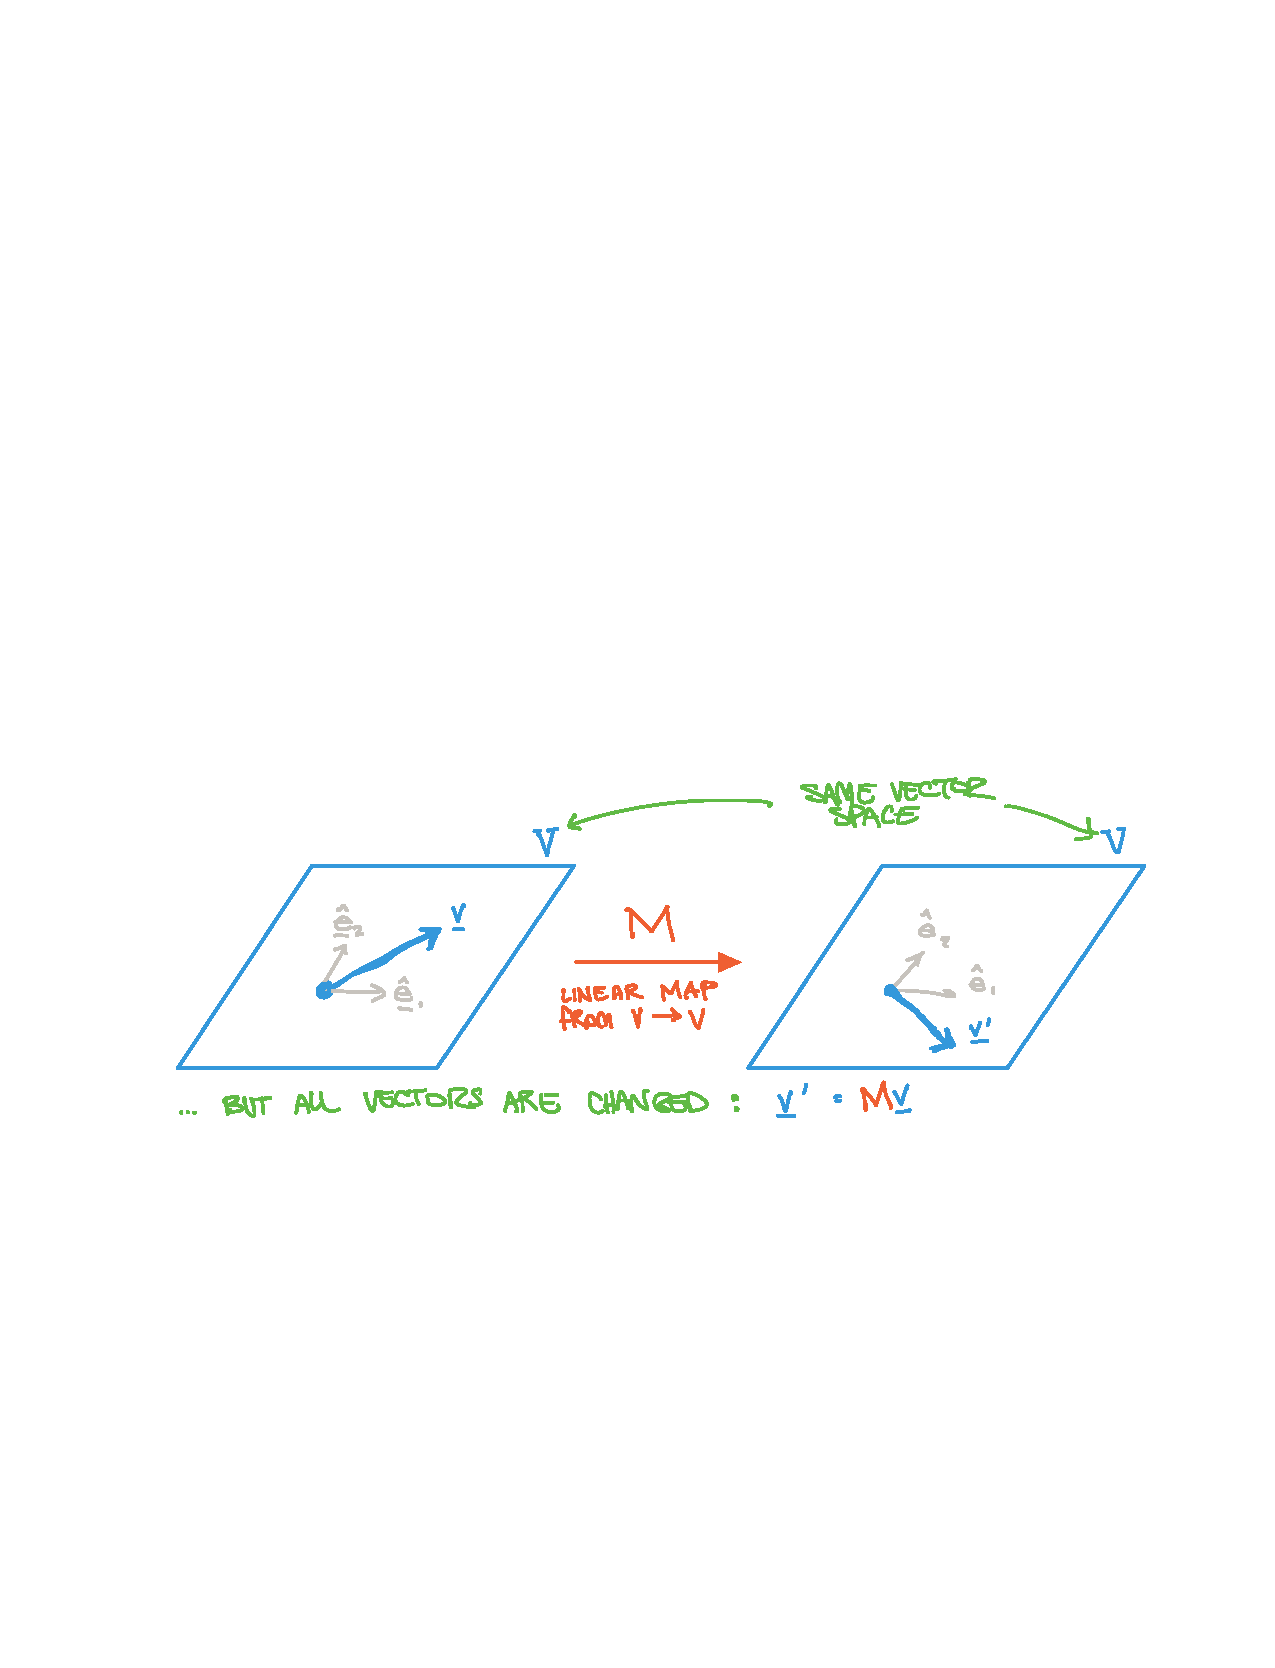
\includegraphics[width=\textwidth]{figures/lineartransformation.pdf}
    \caption{Example of a linear transformation. The transformation $M$ (for matrix) takes a vector $\vec{v}$ and turns it into a different vector that we call $\vec{v}'$. This new vector is related to $\vec{v}$ by the matrix $\vec{v'}=M\vec{v}$. \emph{Every} vector is transformed under the map $M$. This is an \emph{active transformation} where all vectors transform, but the basis ($\hat{\vec{e}}_i$) stays fixed.}
    \label{fig:Linear Transformation}
\end{figure}

\subsection{More Jargon}



Pre-image, image, kernel, 

\subsection{Linear transformations}


% both addition and resscaling are linear

A function $f$ is \textbf{linear} if it satisfies:
\begin{align}
  f(\alpha x) &= \alpha f(x)\\
  f(x+y) &= f(x) + f(y) \ .
\end{align}

\begin{align}
  f(\alpha x + \beta y) = \alpha f(x)+\beta f(y)
  \label{eq:def:linear}
\end{align}



 \section*{Acknowledgments}

\acro{PT}\ thanks the students of Physics 17 (Spring 2022, Spring 2023) for their feedback and patience.
%
% \acro{PT} is supported by the \acro{DOE} grant \acro{DE-SC}/0008541.
\acro{PT} is supported by a \acro{NSF CAREER} award (\#2045333).

%% Appendices
% \appendix


%% Bibliography
%\bibliographystyle{utcaps} 	% arXiv hyperlinks, preserves caps in title
%\bibliographystyle{utphys} 	% arXiv hyperlinks
% \bibliography{bib title without .bib}

\end{document}